\section{Testing}

The demodulation algorithm was tested by coding the algorithm in C (as a console
application) and instrumenting it to display variables,
save arrays to files, and benchmark the various stages.
KissFFT is used as the FFT. A GPU would be much faster and will be used in further studies.

\subsection{Demodulation}

The demodulation algorithm looks at the signal bandwidth between about
$F_S/5$ and $F_S/2$.
Many data sets have a region of interest far below the sample rate.

Decimation may be used to lower the sample rate to bring it to the
desired region of interest. 
Decimation by a factor of $m$ involves low-pass filtering the signal
and taking every $m$th data point as output.

Figure \ref{fig:chirpTest1} shows a spectrogram image of a noisy test signal with R on the vertical axis.
$R=-0.2$ is at the top and $R=-0.78$ is at the bottom.
The output rates for each R are normalized (stretched at the low end) to fit the image.
This gives the top of the image a fuzzy appearance.
A test signal was used to demonstrate detection of a chirp at $R=-0.5$ and $N=4096$.
The chirp amplitude is 1/10 of the noise amplitude.

\begin{figure}
  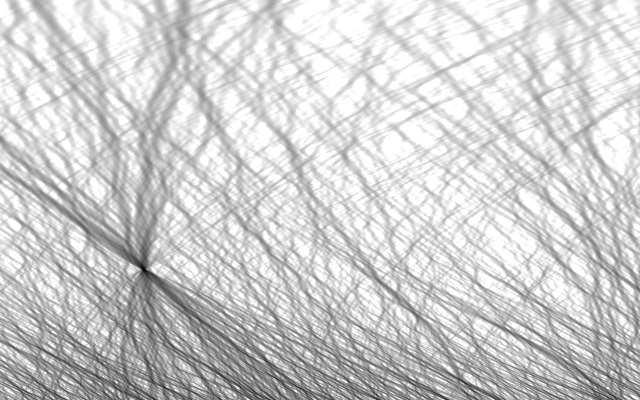
\includegraphics[width=\linewidth]{../source/chirp42m.jpg}
  \caption{Chirp power 20dB below noise.}
  \label{fig:chirpTest1}
\end{figure}

Noise has a cobweb-like look. A chirp shows up as a peak among the cobwebs.
To pick the chirp out of this mess, the peak and RMS values are stored for each R value.
